\documentclass[11pt]{beamer}
\usetheme{Boadilla}
\usepackage[utf8]{inputenc}
\usepackage[english]{babel}
\usepackage[T1]{fontenc}
\usepackage{amsmath}
\usepackage{amsfonts}
\usepackage{amssymb}
\usepackage{tabularx}
\usepackage{graphicx}
\usepackage{url}
\usepackage{mathrsfs}
\usepackage[toc,page]{appendix}
\usepackage{enumitem}
\usepackage{dsfont}

\title{Introduction to neural ODE}
\author{Della Bona Sarah, Dumez Erika}
\date{\today}
\begin{document}

\AtBeginSubsection[]{
\begin{frame}
\tableofcontents[ 
    currentsubsection, 
    hideothersubsections, 
    sectionstyle=show/shaded, 
    subsectionstyle=show/hide
    ]

\end{frame}}

\AtBeginSection[]{
\begin{frame}
\tableofcontents[ 
    currentsection, 
    hideothersubsections, 
    sectionstyle=show/shaded, 
    subsectionstyle=show/hide
    ]

\end{frame}}

\begin{frame}
\titlepage
\end{frame}

\begin{frame}
\tableofcontents[hidesubsections]
\end{frame}

\section{Introduction}
\begin{frame}{What are ODE-Nets?}

\begin{itemize}
\item[•] ODE-Nets are deep neural networks models using ordinary differential equations;
\item[•] Unlike classical neural networks, the hidden layer in an ODE-Net is defined as a black box that uses an ODE solver;
\item[•] They have multiple advantages: constant memory cost, better results in continuous time series data and they are sometime more natural to use.
\end{itemize}

~

The code use to make the examples can be found at \url{https://github.com/DumezErika/ProjetMachineLearning}.
\end{frame}



\section{Machine learning}
\begin{frame}{Machine Learning problem}
In a typical machine learning problem \cite{7}, we have an output variable $Y$ to $p$ predictors $X_1,\dots, X_p$, also called input variable, where $p\in \mathbb{N}\backslash \{0\}$. 

~
\begin{itemize}
\item[•] The inputs belongs to an input space $\mathcal{X}$ and usually $\mathcal{X} \subset \mathbb{R}^p$. 

\item[•] The output belongs to a output space $\mathcal{Y}$. 
\begin{itemize}
\item[•] If this is a regression problem, $\mathcal{Y} \subset \mathbb{R}$;
\item[•] If we have a classification problem with $K$ categories, $\mathcal{Y} = \{1,2,\dots, K\}$.
\end{itemize}
\end{itemize}


\end{frame}

\begin{frame}{Machine Learning problem}
Let's assume that there is some relationship between $Y$ and $X = (X_1,\dots, X_p)$, which can be written in the general form
$$
Y = f(X) + \epsilon.
$$
Where $f$ is some fixed but unknown function, called \textit{target function}, of $X_1, \dots, X_p$ and $\epsilon$ is a random error term which is independent of $X$ and has mean zero and finite variance.

\end{frame}

\begin{frame}{Machine Learning problem}

The goal of supervised learning is to estimate this function $f$ as precisely as possible using a model that we will train. To do that, we need a \textit{data set} to learn. The data is a set of $n$ points in $\mathcal{X} \times \mathcal{Y}$
$$
\mathcal{D} = \{(x_1, y_1),\dots, (x_n,y_n)\}.
$$

~

Let $x$ be a data point, then we can predict its output $y$ using 
$$
\hat{y} = \hat{f}(x),
$$
where $\hat{f}$ represents our estimate for $f$, and $\hat{y}$ represents the resulting prediction for $y$.
\end{frame}

\begin{frame}{Machine Learning Problem}
To determine the precision of an estimation $\hat{f}$, we use a \textit{loss function}. Some example of loss functions are
\begin{itemize}
\item[•] Square error loss: $\mathcal{L}(y, \hat{y}) = (y-\hat{y})^2$;
\item[•] Absolute error loss: $\mathcal{L}(y, \hat{y}) = |y - \hat{y}|$;
\item[•] Zero-one loss: $\mathcal{L}(y, \hat{y}) = \mathds{1}_{\{(y, \hat{y}) | y\neq \hat{y}\}}(y, \hat{y})$.
\end{itemize}
\end{frame}

\begin{frame}{Machine Learning Problem}
\begin{itemize}
\item[•] \textbf{Training : } 

To train the model we use a data set called the \textit{train set}. The model is
constructed with different parameters $\theta$. During the training we search for the
parameters that will minimize the chosen loss function. 
\item[•] \textbf{Testing : } 

Once the model is trained, we can test it on an other data set, called the test set, using an
error measure which can be a loss function. The error on the test set is called
\textit{out-of-sample error} whereas the error on the training set is called the \textit{in-sample
error}.
\end{itemize}
\end{frame}

\subsection{Neural Networks}
\begin{frame}{Neural Network}
\begin{definition}
A \textit{neural network} \cite{5} can be used to solve a machine learning problem. It consists of a series of layers. There are three types of layers :

\begin{itemize}
\item[•] The \textit{input} layer
\item[•] The \textit{output} layer
\item[•] The \textit{hidden} layers
\end{itemize}
Each layer consist of a certain number of neurons. We give an input $x$ to the neurons of a layer, they do some calculus and give an output $z$.

~

An \textit{activation function} is then applied to this output and obtain a value $h$ before transmitting it to the next layer thanks to the connections between the neurons of each layer.
\end{definition}
\end{frame}

\begin{frame}{Examples}
Some example of activation function are:
\begin{itemize}
\item[•] Hyperbolic tangent : $\tanh(z) = \frac{e^z - e^{-z}}{e^z + e^{-z}}$;

\item[•] Sigmoid : $sigmoid(z) = \frac{1}{1 + e^{-z}}$;
\item[•] ReLU : $ReLU(z) = \max(0,z)$;
\item[•] Sign : $sign(z) = \begin{cases}
1 \text{ if z > 0},\\
0 \text{ if z = 0},\\
-1 \text{ else}.
\end{cases}$
\end{itemize}

~

The simplest example of a neural network layer is 
$$
h = \sigma (Wx +b)
$$
where $\sigma$ is an activation function, $W$ is a weight matrix and $b$ a bias vector.
\end{frame}

\begin{frame}{Forward and Backward Pass}

\begin{center}
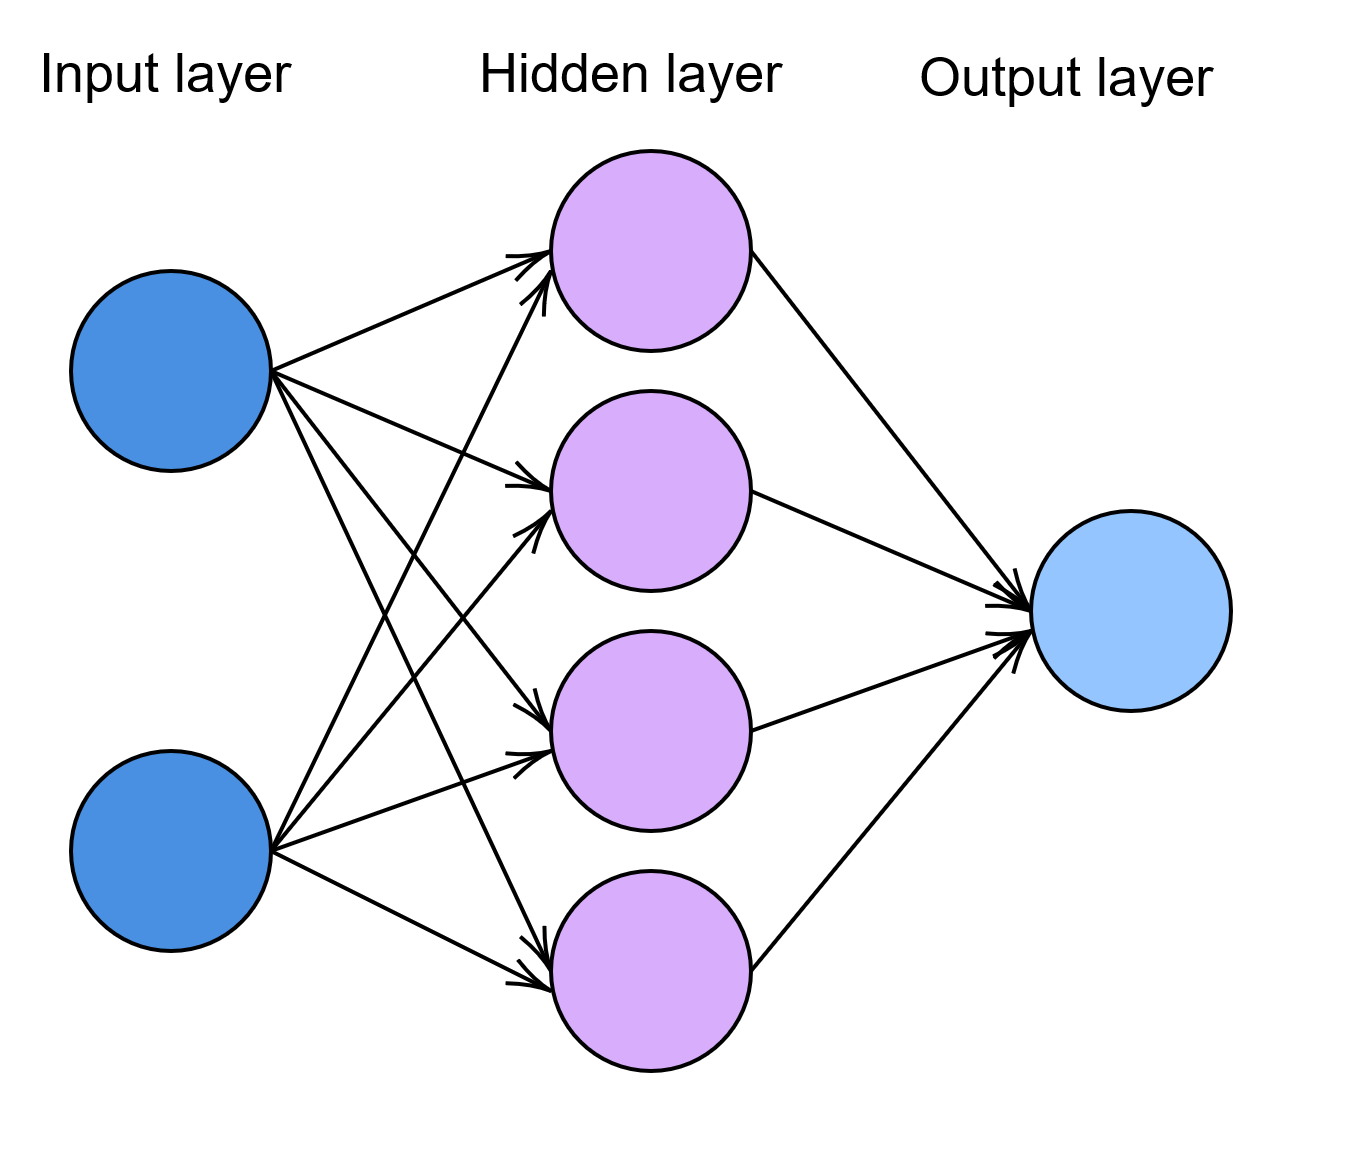
\includegraphics[scale=0.14]{nn.png}
\end{center}


The goal is to minimize the training error for every input of the training set. To do that, we need to find the optimal parameters for the network which minimize the loss function. We need to compute the derivatives of the loss with respect to the parameters.
\end{frame}

\subsection{Back propagation}
\begin{frame}{Back propagation}
Let $\theta$ be the parameters of the network. We want to find $\theta^*$ which minimize the loss function in order to have the in-sample error as small as possible. 

~

We want to determine the partial derivatives of the loss function with respect to the parameters, $\frac{\partial \mathcal{L}}{\partial \theta}$, and find $\theta^*$ such that these derivatives are $0$.

~

\textit{Backpropagation} \cite{11} is the process used to compute this derivatives. It works by computing the gradient of the loss function with respect to each parameter by the chain rule, computing the gradient one layer at a time, iterating backward from the final layer.
\end{frame}

\subsection{Gradient descent}
\begin{frame}{Gradient Descent}
\textit{Gradient descent} \cite{1} is a process used to approximate a local minimum of a differentiable function. 

It works as follows: at each step of the process, we take a step in the opposite direction of the gradient of the function at the current point.

~

More formally, if we have a function $g: \mathbb{R}^m \rightarrow \mathbb{R}$, $m>1$, differentiable and a point $x_0\in \mathbb{R}^m$, we have that if
$$
x_{n+1} = x_n -\gamma_n \nabla g(x_n), n\geq 0
$$
for $\gamma_n \in \mathbb{R}^+$ small enough, then $g(x_n) \geq g(x_{n+1})$. 

\end{frame}

\subsection{Residual neural network} \label{rnn}
\begin{frame}{Residual neural network}

A\textit{ residual neural network} \cite{6}, also called ResNet, is a neural network which has more connections. Indeed, a layer receives as input the outputs of the previous layer and its inputs.

 \begin{columns}[t]
  \begin{column}{5cm}
\begin{center}
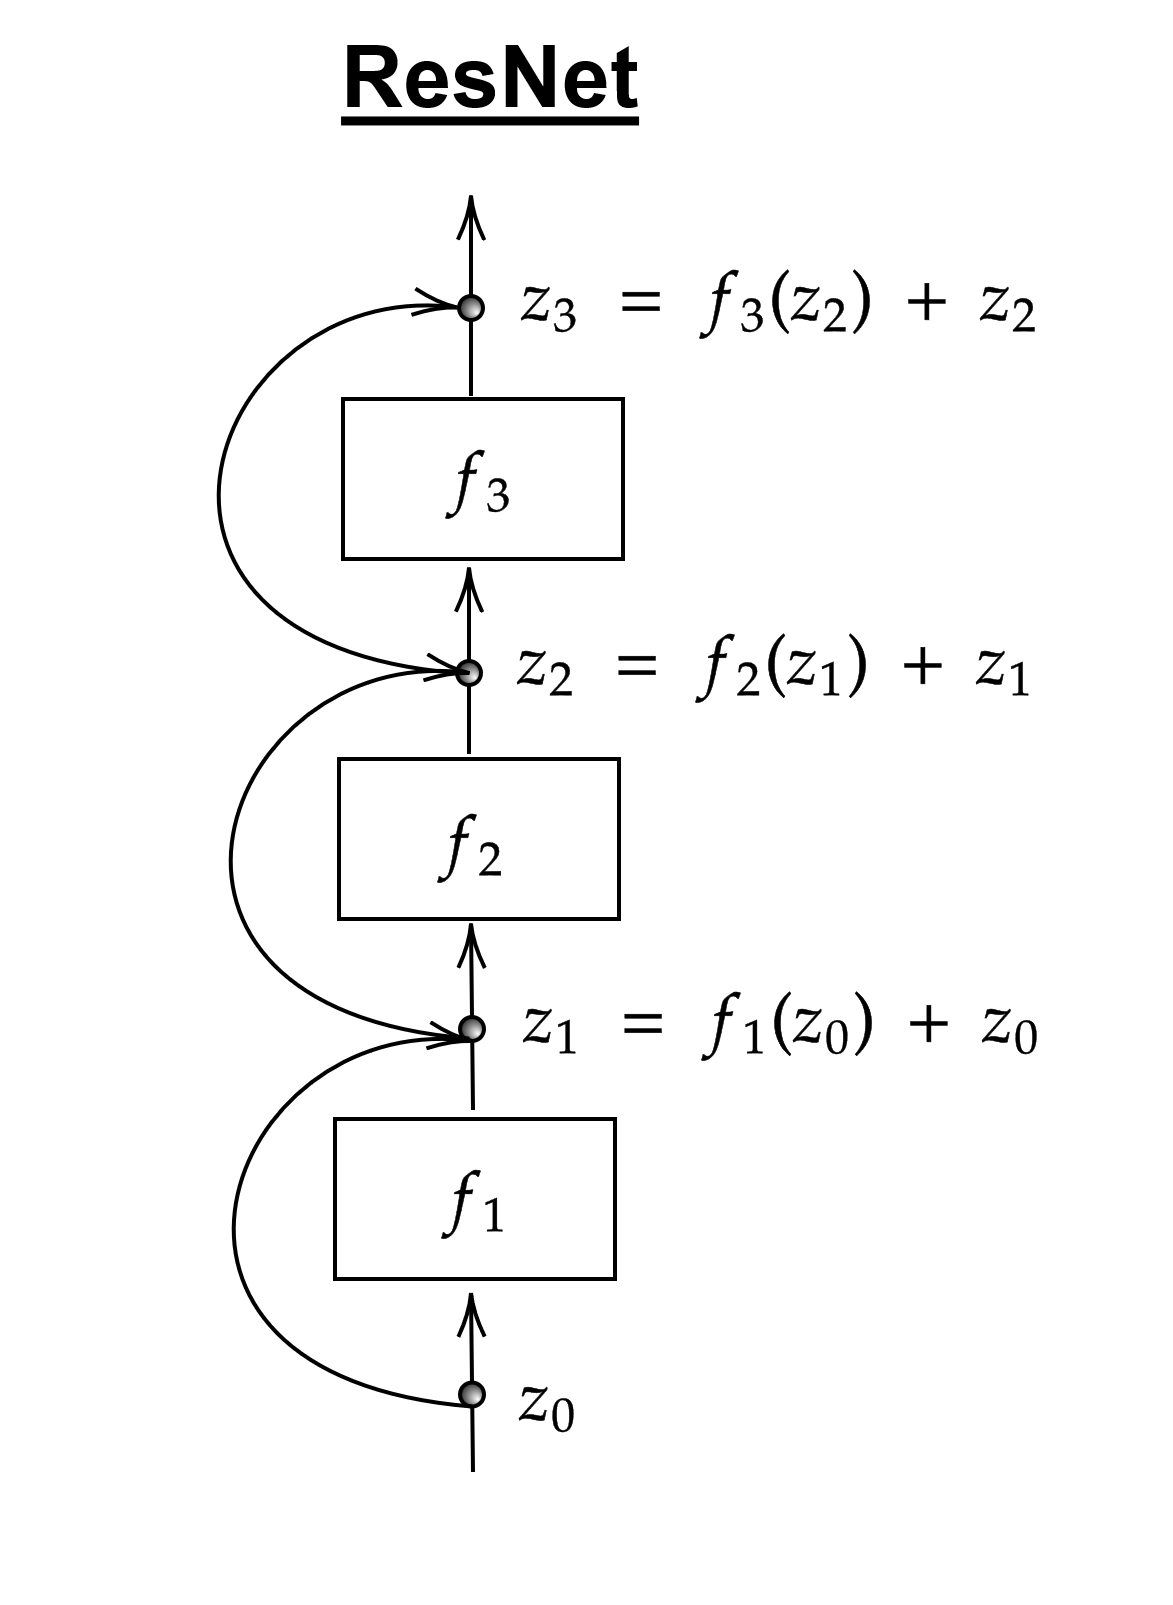
\includegraphics[scale=0.14]{resnet.png}
\end{center}
  \end{column}
  
  \begin{column}{5cm}
  \begin{center}
  ~
  
  ~
  
  ~
  
  
  In these networks, the output of the $k+1$th layer is given by
$
z_{k+1} = z_k + f_k(z_k)
$,
where $f_k$ is the function of the $k$th layer and its activation. 
  \end{center}

  \end{column}
 \end{columns} 
\end{frame}

\section{Ordinary Differential Equations}
\begin{frame}{First Order Ordinary Differential Equations}
An\textit{ ordinary differential equation} (ODE) \cite{9} is an equation that describes the changes of a function through time. The goal is to compute that function from the ODE which describes its derivative. In this setting, time is a continuous variable.

\begin{definition}
Let $\Omega \subseteq \mathbb{R} \times \mathbb{R}^N$ an open set. Let $f: \Omega \rightarrow \mathbb{R}^N$. 

A \textit{first order ODE} takes the form
$$
\frac{\partial u}{\partial t}(t) = f(t,u(t))
$$
\end{definition}
\end{frame}

\begin{frame}{Solution of ODE's}
\begin{definition}
A \textit{solution} for this ODE is a function $u : I \rightarrow \mathbb{R}^N$, where $I$ is an interval, such that
	\begin{itemize}
	\item[•] $u$ is differentiable on $I$,
	\item[•] $\forall t \in I, (t, u(t)) \in \Omega$,
	\item[•] $\forall t \in I, \frac{\partial u}{\partial t}(t) = f(t, u(t))$
	\end{itemize}
\end{definition}
\end{frame}

\begin{frame}{Cauchy Problems}

\begin{definition}
An \textit{initial condition} (IC) is a condition of the type
$$
u(t_0) = u_0
$$
where $(t_0, u_0) \in \Omega$ is given.
\end{definition}

\begin{definition}
A \textit{Cauchy problem} is an ODE with IC
$$
\left \{
\begin{array}{rcl}
\frac{\partial u}{\partial t}(t) & = & f(t, u(t)) \\
u(t_0) & = & u_0
\end{array}
\right.
$$
\end{definition}
\end{frame}

\subsection{One-step methods}
\begin{frame}{One-step methods}
It is not always possible to explicitly find a solution to a Cauchy problem. 

~

However, let $T > 0$ such that the solution $u$ exists on $[t_0, t_0 + T]$ and let $n \geqslant 2$ be a natural. Let  $t_0 < ... < t_n \in [t_0, t_0 + T]$ where $t_n = t_0 + T$. We obtain a finite number of points $(u_0, \dots, u_n)$ such that:
$$
\forall i\in \{0,\dots, n\},  u_i \approx u(t_i).
$$

To compute those points, we use \textit{one-step methods} which compute the points $u_{i+1}$ from the previous point $u_i$, the time $t_i$ and the \textit{step} $h_i := t_{i+1} - t_i$.
\end{frame}

\subsection{Euler's method} \label{euler}
\begin{frame}{Euler's Method}
Euler's method is a one-step method with a constant step $h$. 

It is similar to a Taylor development, the idea is to compute $u(t_{i+1})$ using the formula
\begin{equation}\label{eqeuler}
u(t_{i+1}) \approx u(t_i) + h\frac{\partial u}{\partial t}(t_i)
\end{equation}
where 
$$
\frac{\partial u}{\partial t}(t_i) = f(t_i, u(t_i)).
$$
for a function $f$.
\end{frame}

\begin{frame}{ResNets and Euler}
If we look back at the formula in the ResNet, we can see
that this is a special case of the formula for Euler method
\begin{equation*}
z_{k+1} = z_k + hf_k(z_k),
\end{equation*}
when $h = 1$.

\end{frame}

\section{Neural ODE} \label{neuralode}
\subsection{Introduction}

\begin{frame}{Explicit and implicit layers}
There is two different ways to define a layer : \textit{explicitly} or \textit{implicitly} \cite{2}. When we define a layer explicitly, we specify the exact sequence of operations to do from the input to the output layer. 

~

We can also define them implicitly: we specify the condition we want the layer's output to satisfy. 

\begin{definition}
An \textit{explicit layer} is defined by a function $f : \mathcal{X} \rightarrow \mathcal{Y}$. For an \textit{implicit layer}, we give a condition that a function $g: \mathcal{X} \times \mathcal{Y} \rightarrow \mathbb{R}^n$ should satisfy. For example we can search for a $y$ such that $g(x,y) = 0$.
\end{definition}
\end{frame}

\begin{frame}{Neural ODE}
In a residual neural network, the output for an input $x$ is a composition of functions. We want to extract all these individual layers to only have one "shared" layer.

\begin{definition}
A \textit{neural ODE network} (or ODE-Net) \cite{2,3,12} takes a simple layer as a building block. This “base layer” is going to specify the dynamics of an ODE.

\end{definition}
ODE-Net enable us to replace layers of neural networks with a continuous-depth model.
\end{frame}
\begin{frame}{Comparison with ResNets}

Let us return to ResNets to give intuition behind this definition. 

We know that any output of the $k^{th}$ layer of a residual network can be computed with the function
\begin{equation*}
F(z_t, t; \theta) = f(z_t, t;\theta) + z_t
\end{equation*}
where $t = k - 1$ and $\theta$ represents the parameters of the layers.

~

Thus, in the ResNet, the output for the input $z_0 = x$ is a composition of the functions $F(z_t, t; \theta)$.
\end{frame}

\begin{frame}
\begin{center}
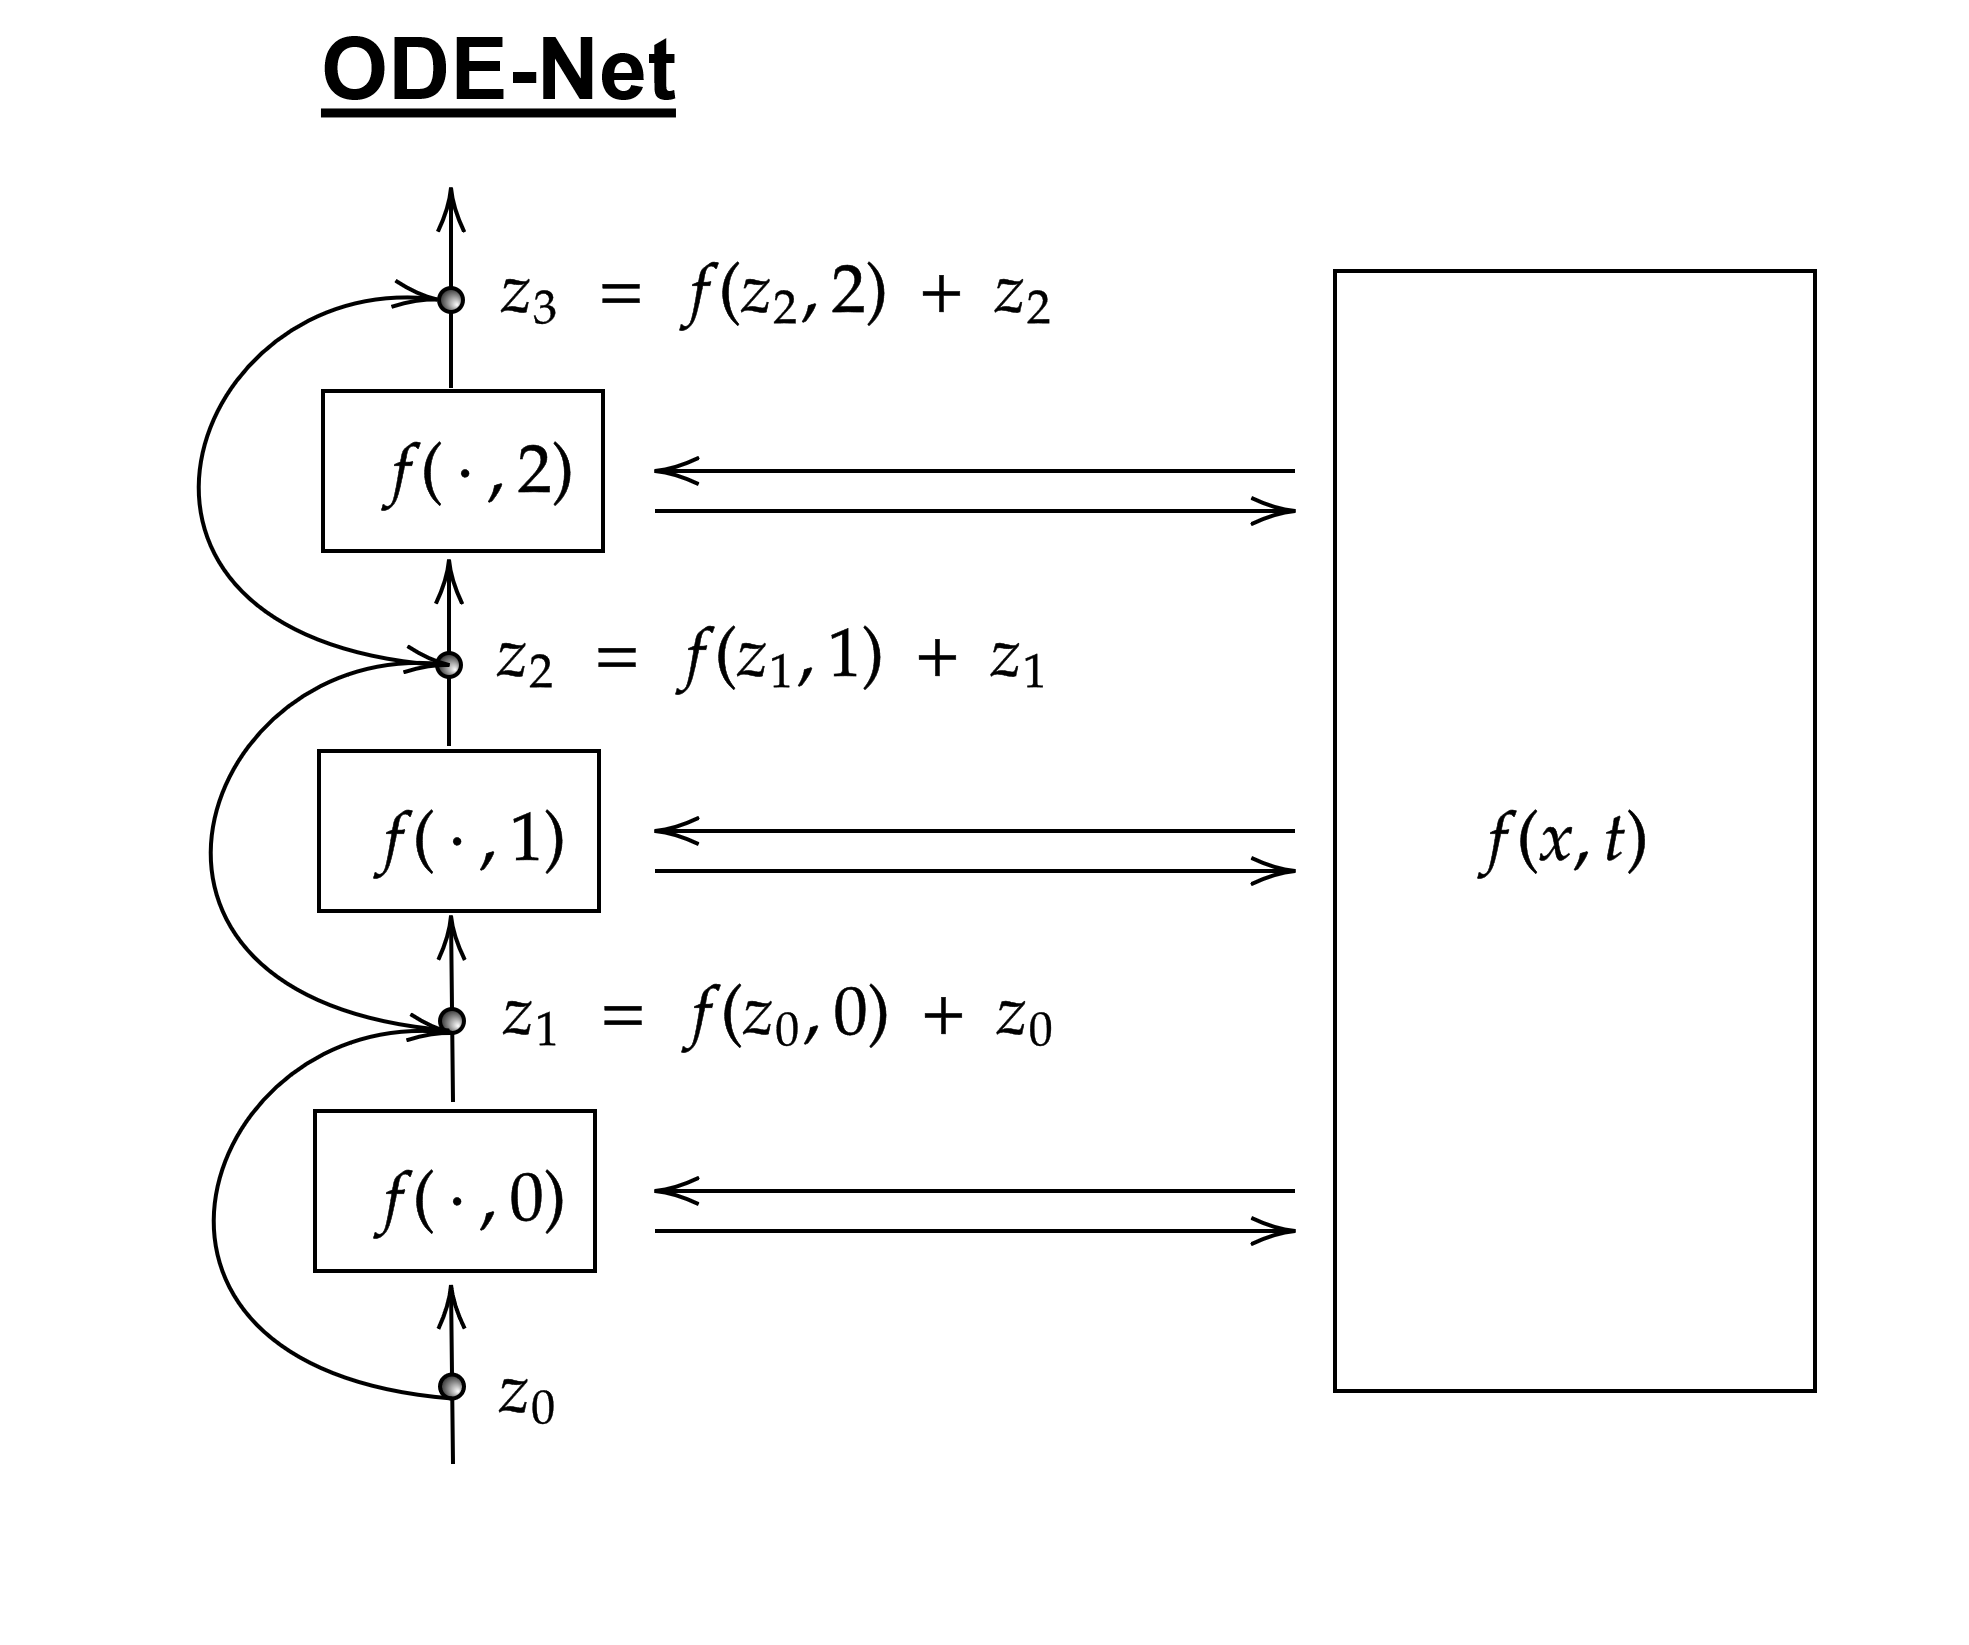
\includegraphics[scale=0.12]{ODENet.png}
\end{center}

We can then view the variables $z_t$ as a function $z$ of $t$. For example,
$
z_1 := z(1) = f(x, 0) + x.
$

~

With that, we can write $F(z_t, t; \theta) = F(z(t), t; \theta)$.
\end{frame}

\begin{frame}
We can see that in ResNets, the outputs of each layer are the solutions of an ODE using Euler's method. The ODE from which it is a solution is $$\frac{\partial z}{\partial t}(t) = f(z(t),t;\theta).$$

~

However, to find the solution to this Cauchy problem, we need the initial value of $z$, which is $z(t_0):=  z_0 = x$. We obtain the following Cauchy problem:
\begin{equation}
\label{cauchypb}
\begin{cases}
\frac{\partial z}{\partial t}(t) =  f(z(t), t; \theta) \\
z(t_0) =  x
\end{cases}
\end{equation}

\end{frame}

\subsection{Forward pass}
\begin{frame}{Forward pass}
The layer in an ODE-Net is implicit. The output $z(t_N)$ of an ODE-Net with the input $z(t_0)$ is defined by the Cauchy problem (\ref{cauchypb}), which depends on the parameters $z(t_0),t_0,\theta$.

~
\begin{center}
But how do we solve this problem?
\end{center}


~

We can use an ODE Solver with the parameters given above.
\end{frame}

\subsection{Backward pass: the Adjoint method}
\begin{frame}{Backward pass}

Now that we know how to compute the output of an ODE-Net, we need a method to find the optimal parameters that minimize the loss function.

~
\begin{itemize}
\item[•] In regular neural networks, we usually use the gradient descent
\item[•] For ODE-Nets, it is more difficult because we used an ODE solver in the forward pass which is some sort of black box.
\end{itemize}

~

This is why we are introducing the \textit{adjoint method} \cite{12}. This method computes the gradient by solving a second ODE backwards and is applicable to all ODE solvers.

\end{frame}
\begin{frame}{Adjoint method}

Let $\mathcal{L}$ be a loss function. To minimize this loss function $\mathcal{L}$, we need gradients with respect to the parameters $z(t_0),t_0,t_N,\theta$. To achieve that, we can determine how the gradient of the loss depends on the hidden state $z(t)$ for each $t$, which is
\begin{equation}
a(t)= \frac{\partial \mathcal{L}}{\partial z(t)}
\end{equation}

This quantity is called the \textbf{adjoint}. We would like to determine its dynamics, so we need to compute its derivative with respect to $t$.

\end{frame}

\begin{frame}{Adjoint method}
With a continuous hidden state, we can write the transformation after an $\varepsilon$ change in time as :
\begin{equation}
\label{zteps}
z(t+\varepsilon) = \int^{t+\varepsilon}_{t} f(z(t),t,\theta) dt + z(t).
\end{equation}
% car f(..) = d(z) et z(1) = z(0) + z(1) - z(0)
Let $ G : \varepsilon \mapsto z(t+\varepsilon)$. We can apply the Chain rule and we have 
\begin{equation*}
\frac{\partial \mathcal{L}}{\partial z(t)} = \frac{\partial \mathcal{L}}{\partial z(t+\varepsilon)} \frac{\partial z(t+\varepsilon)}{\partial z(t)}.
\end{equation*}
In other words 
\begin{equation}
\label{at}
a(t) = a(t+\varepsilon)\frac{\partial G(\varepsilon)}{\partial z(t)}.
\end{equation}
\end{frame}

\begin{frame}{Adjoint method}
\begin{eqnarray*}
\frac{\partial a}{\partial t}(t) &=& \lim_{\varepsilon \rightarrow 0^+} \frac{a(t+\varepsilon) - a(t)}{\varepsilon}\\
&=& \lim_{\varepsilon \rightarrow 0^+} \frac{a(t+\varepsilon) - a(t+\varepsilon)\frac{\partial G(\varepsilon)}{\partial z(t)}}{\varepsilon}\\
&=& \lim_{\varepsilon \rightarrow 0^+} \frac{a(t+\varepsilon) - a(t+\varepsilon)\frac{\partial z(t) + \varepsilon f(z(t),t,\theta) + O(\varepsilon^2)}{\partial z(t)}}{\varepsilon} \\
&=& \lim_{\varepsilon \rightarrow 0^+} \frac{a(t+\varepsilon) - a(t+\varepsilon)(\mathds{1} + \varepsilon \frac{\partial f(z(t),t,\theta)} {\partial z(t)}+ O(\varepsilon^2))}{\varepsilon}\\
&=& \lim_{\varepsilon \rightarrow 0^+} \frac{-\varepsilon a(t+\varepsilon) \frac{\partial f(z(t),t,\theta)} {\partial z(t)}+ O(\varepsilon^2)}{\varepsilon}\\
&=& -a(t)\frac{\partial f(z(t),t;\theta)} {\partial z(t)}
\end{eqnarray*}
\end{frame}

\begin{frame}{Adjoint method}
We now have the dynamics of $a(t)$
\begin{equation}
\label{dynat}
\frac{\partial a(t)}{\partial t} = -a(t)\frac{\partial f(z(t),t;\theta)} {\partial z(t)}
\end{equation}
 
As we are searching for $ a(t_0) = \frac{\partial \mathcal{L}}{\partial z(t_0)}$, we need to solve an ODE for the adjoint backwards in time because the value for $a(t_N)$ is already known. The constraint on the last time point, which is simply the gradient of the loss with respect to $z(t_N)$, 
\begin{equation*}
a(t_N) = \frac{\partial \mathcal{L}}{\partial z(t_N)},
\end{equation*}
has to be specified to the ODE solver. 
\end{frame}

\begin{frame}{Adjoint method}
Then, the gradients with respect to the hidden state can be calculated at any time, including the initial value. 

~

If we want to compute the gradient with respect to the parameters $\theta$, we have to evaluate another integral, which depends on both $z(t)$ and $a(t)$,
\begin{equation}
\label{devtheta}
\frac{\partial \mathcal{L}}{\partial \theta} = - \int^{t_0}_{t_N} a(t) \frac{\partial f(z(t),t;\theta)} {\partial \theta} dt.
\end{equation}
\end{frame}

\begin{frame}{Adjoint method}
To avoid computing each ODE on its own, we can do all of them at the same time. To do that we can generalize the ODE to
\begin{eqnarray*}
\frac{\partial}{\partial t} \begin{bmatrix}
							z \\ \theta \\ t
							\end{bmatrix} (t) 
= f_{aug}([z(t),\theta ,t]) := \begin{bmatrix}
							f([z(t),\theta ,t]) \\ 0 \\ 1
							\end{bmatrix}, \\
a_{aug} (t) := \begin{bmatrix}
			a \\ a_{\theta} \\ a_t
			\end{bmatrix} (t) , \ 
a(t) = \frac{\partial \mathcal{L}}{\partial z(t)}, \ 
a_\theta (t) = \frac{\partial \mathcal{L}}{\partial \theta (t)}, \ 
a_t(t) := \frac{\partial \mathcal{L}}{\partial t(t)}.
\end{eqnarray*}
\end{frame}

\begin{frame}{Adjoint method}
The jacobian of $f_{aug}$ has the form
\begin{equation*}
\frac{\partial f_{aug}}{\partial [z(t),\theta,t]}([z(t),\theta,t]) = \begin{bmatrix}
\frac{\partial f}{\partial z} & \frac{\partial f}{\partial \theta} & \frac{\partial f}{\partial t} \\
\textbf{0} & \textbf{0} & \textbf{0} \\
\textbf{0} & \textbf{0} & \textbf{0}
\end{bmatrix}(t)
\end{equation*}

where each \textbf{0} is a matrix of zeros with the corresponding dimensions.

We can inject $a_{aug}$ in (\ref{dynat}) and we get
\begin{eqnarray*}
\frac{\partial a_{aug}(t)}{\partial t} 
&=& - [a(t) \ a_\theta (t) \ a_t (t)]\frac{\partial f_{aug}}{\partial [ z(t),\theta , t]}([z(t),\theta , t]) \\
&=& -\Big[a\frac{\partial f}{\partial z} \ a\frac{\partial f}{\partial \theta} \ a\frac{\partial  f}{\partial t}\Big] (t).
\end{eqnarray*}
\end{frame}

\begin{frame}{Adjoint method}
We can also get gradients with respect to $t_0$ and $t_N$ by integrating the last component, $-a(t)\frac{\partial f(z(t),t;\theta)}{\partial t(t)}$, and by using the Chain rule. 

We have
\begin{eqnarray*}
\frac{\partial \mathcal{L}}{\partial t_0} &=& a_t(t_0) = a_t(t_N) - \int_{t_N}^{t_0} a(t) \frac{\partial f(z(t),t,\theta)}{\partial t} dt ; \\
\frac{\partial \mathcal{L}}{\partial t_N} &=& \frac{\partial \mathcal{L}}{\partial z(t_N)} \frac{\partial z(t_N)}{\partial t_N} = a(t_N)f(z(t_N),t_N,\theta).
\end{eqnarray*}
With this generalized method, we have gradients for all possible inputs to a Cauchy problem solver. 
\end{frame}

\section{Simulated Data}

\begin{frame}{Approximating a function}

Let $h:\mathbb{R} \to \mathbb{R}$ be a function such that
$$
h(x) = x^3 + 0.1x.
$$
We can train a ResNet and an ODE-Net to approximate this function.

To do that, we need a training set of points. We generate $10$ points between $-2.5$ and $2.5$. Their associated output comes from the function
$$
h(x) + \varepsilon,
$$
where $\varepsilon$ is a noise variable with mean $0$ and standard deviation $1$.
\end{frame}

\begin{frame}{ResNet}

We train a ResNet with $3$ layers, the hidden one having $20$ neurons. Each layer has the hyperbolic tangent as activation function. The step-size used during training was $0.01$. After $1000$ iterations we get the following result.


\begin{center}
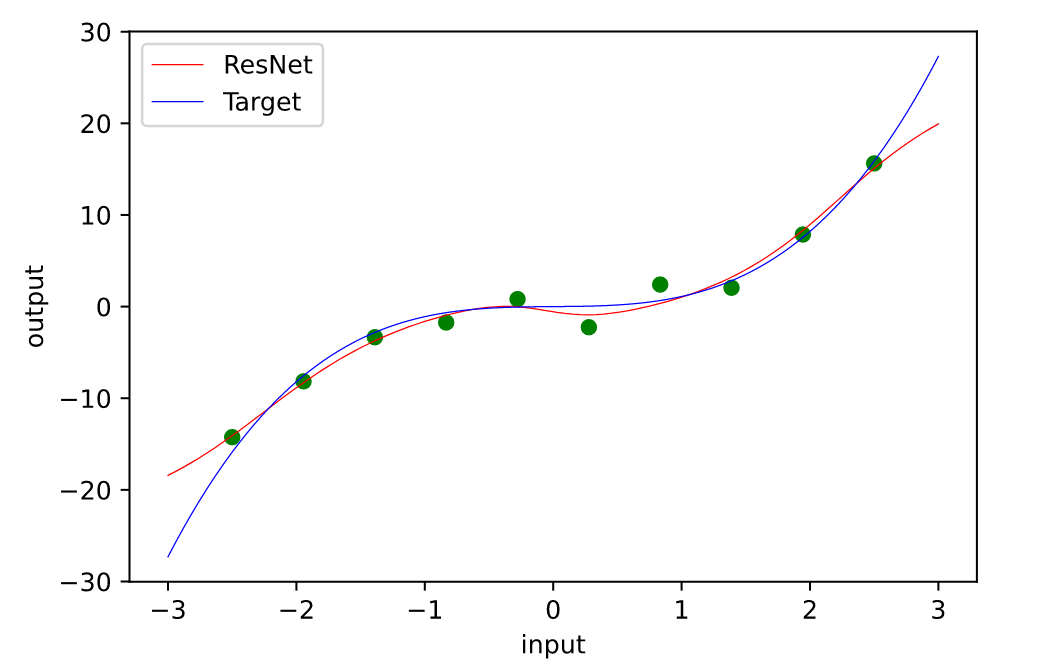
\includegraphics[scale=0.4]{ex_resnet.png}
\end{center}

With the mean squared error, the out-of-sample error for the points used to trace the line is $4.673$.
\end{frame}

\begin{frame}{ODE-Net}

The dynamics of the ODE-Net is specified by a layer of size $20$. The step-size in this case is $0.005$, each layer has also the hyperbolic tangent. After $1000$ iterations, we get the function given in this figure.

\begin{center}
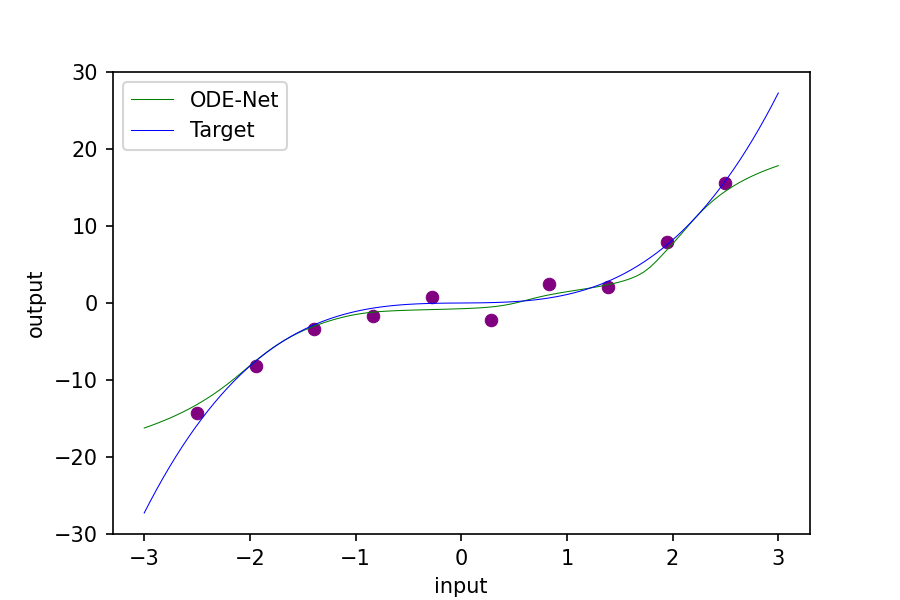
\includegraphics[scale=0.45]{ex_odenet_final.png}
\end{center}

The out-of-sample error for the same points is $7.72$.
\end{frame}

\begin{frame}{Comparison}
When we compare the result of both models, we can see that the ResNet is slightly better with these parameters.
\begin{center}
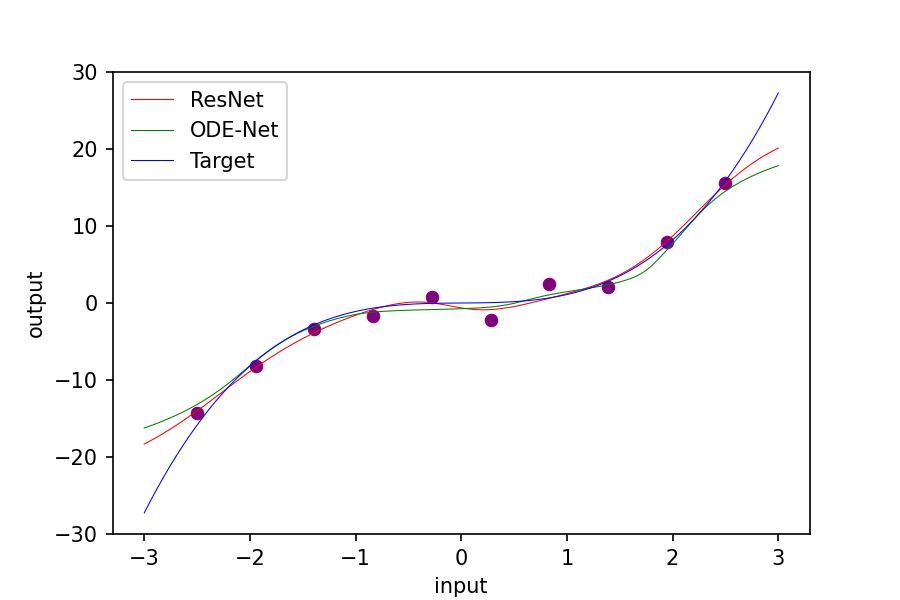
\includegraphics[scale=0.45]{comparaison_final.png}
\end{center}
\end{frame}

\section{Example with real data}
\begin{frame}{Electrocardiogram dataset}
Now that we tested the ODE-Net architecture on a small example, we can test it on real data to see how it performs.

~

The data we chose is the MIT Beth Israel Hospital (BIH) electrocardiogram dataset that can be found at \url{https://www.kaggle.com/shayanfazeli/heartbeat}. 

It contains two data sets: one for training and one for testiong.
\end{frame}

\begin{frame}{Electrocardiogram dataset}
The training data set consists of around $90,000$ samples, classified as either
\begin{itemize}
\item[•] 0: normal;
\item[•] 1: supraventricular premature beat;
\item[•] 2: premature ventricular contraction;
\item[•] 3: fusion of ventricular and normal beat;
\item[•] 4: unclassified beat;
\end{itemize}
and the test data set is composed similarly, with around $20,000$ samples.
\end{frame}

\begin{frame}{Architecture of the models}
We will build a ResNet and a ODE-Net as similar as possible so that we can compare them better.

~

\begin{itemize}
\item[•] The ResNet is composed of $3$ firstlayers with ReLU as activation function, followed by $6$ residual blocks also with ReLU. The output layer is a simple layer;
\item[•] The ODE-Net is composed similarly of $3$ first layers, each followed by the activation function ReLU. The dynamics are defined by a layer taking time into account. The output layer is the same as for the ResNet, i.e. a simple layer.
\end{itemize}
\end{frame}

\begin{frame}{Architecture of the models}
To optimize our model we use the cross entropy error. The parameters are then updated using stochastic gradient descent with a step-size of $0.1$ and a momentum of $0.9$. 

~

Stochastic Gradient Descent with momentum is a method that accelerate the computation of the gradient and thus leads to faster converging \cite{8}.

~

We trained each models on the training set for $25$ epochs with batches of size $128$. 
\end{frame}

\begin{frame}{Results for the ResNet}
In this figure we can see the evolution of the training and testing error of the ResNet. We tested our models on the test data set and used the cross entropy error to evaluate it. At the end of training, the ResNet had a test error of $0.1$.
\begin{center}
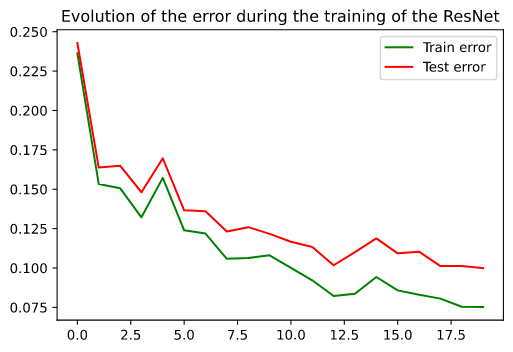
\includegraphics[scale=0.4]{resnet_rd_loss.png}
\end{center}

\end{frame}

\begin{frame}{Results for the ODE-Net}
In this figure we can see the evolution of the training and testing error of the ODE-Net. At the end of training, the ODE-Net had a test error of $0.09$.
\begin{center}
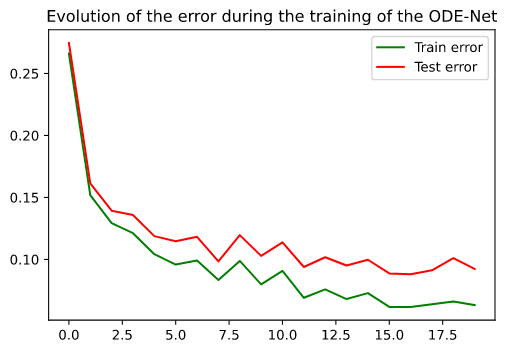
\includegraphics[scale=0.4]{odenet_rd_loss.png}
\end{center}
Therefore, the ODE-Net performs slightly better than the ResNet and the figures show that the ODE-Net learns faster since the curve decreases in less epochs.
\end{frame}

\begin{frame}{Comparison of the models}
We also computed the accuracy of each models. To do so we first used softmax to compute predictions for the test data, then we used the zero-one loss on those predictions. The ResNet has an accuracy of $97.5\%$ while the ODE-Net has a slightly better accuracy of $97.8\%$.

~

Another way of judging the quality of a model in the case of classification is to look at its \textit{confusion matrix}.
\end{frame}

\begin{frame}{Confusion matrices}
Here are the confusion matrices of our models.

~

\begin{columns}
\begin{column}{5cm}
\begin{center}
ResNet:
  
$$
\begin{pmatrix}
18056 & 12 & 36 & 5 & 9 \\
209 & 339 & 5 & 1 & 2 \\
99 & 8 & 1313 & 23 & 5 \\
52 & 0 & 16 & 94 & 0 \\
47 & 0 & 10 & 0 & 1551
\end{pmatrix}
$$
\end{center}

\end{column}
\begin{column}{5cm}
\begin{center}
ODE-Net :
  
$$
\begin{pmatrix}
17989 & 43 & 74 & 3 & 9 \\
151 & 389 & 15 & 0 & 1 \\
59 & 2 & 1376 & 10 & 1 \\
36 & 0 & 26 & 100 & 0 \\
36 & 0 & 16 & 0 & 1556
\end{pmatrix}.
$$
\end{center}
\end{column}
\end{columns} 

\end{frame}

\section{Advantages and disadvantages of ODE-Nets}
\subsection*{Advantages}

\begin{frame}{Advantages}
\begin{itemize}
\item[•] \textit{ODE solvers}

We can use ordinary differential equations solvers instead of gradient descent. These solvers have more than a hundred years of theory behind them which is a great advantage against gradient descent.
\end{itemize}
\end{frame}

\begin{frame}{Advantages}
\begin{itemize}
\item[•] \textit{Robustness} \cite{4}

It was proved that ODE-Net are very robust against perturbed data compared to regular neural network. 

Two experiments were conducted: in the first one they trained an ODE-Net and a convolutional neural network\footnote{A neural network that is usually good with images.} on real images without perturbations. They tested these models on the original images and the ODE-Net outperformed the CNN. In the second experiment, they trained these networks on the original and perturbed images. Again, the ODE-Net was much better.
\end{itemize}
\end{frame}

\begin{frame}{Advantages}
\begin{itemize}
\item[•] \textit{Constant memory cost}

There's a constant memory cost, instead of increasing the cost linearly with each layer in a regular network. 

In ODE-Net, we know the state at every time $t$. Because of that, we can always reconstruct the entire trajectory of an ODE forwards and backwards in time only by knowing this point. This means that ODE-Nets can be trained with a memory cost constant in the number of evaluations of $f$.
There is a trade-off between memory cost and computational time: ResNets are faster but use more memory and ODE-Net are slower but use less memory.
\end{itemize}
\end{frame}

\begin{frame}{Advantages}
\begin{itemize}
\item[•] \textit{Continuous time series predictions}

The biggest advantage of ODE-Nets is that they have more accurate results for time series predictions. Regular neural network have discrete layers, which means they expect the intervals for these time series data sets to be fixed whereas ODE-Net have a continuous layer which means we can evaluate the hidden states at every point $t$ in time. Therefore, regular neural networks are bad at predicting output for time series data that is irregular.
\end{itemize}
\end{frame}

\begin{frame}{Disadvantages}
\begin{itemize}
\item[•] \textit{Slower training time}

ODE-Net have a slower training time. Indeed, during training, the dynamics we want to learn tend to become expensive to solve since the network becomes deeper. However, regular neural networks can be evaluated with a fixed amount of computation, and are typically faster to train. In this case, we don't have to choose an error tolerance for a solver.

There is then a trade-off between accuracy and computational time: if we choose a small error tolerance, then the computational time be bigger.
\end{itemize}
\end{frame}

\begin{frame}{Disadvantages}
\begin{itemize}
\item[•] \textit{More Hyperparameters}

In ODE-Nets we need to choose a solver and its error tolerance, which induces more choices to find the parameters which works better.
\end{itemize}
\end{frame}


\section{References}


\begin{frame}[allowframebreaks]

\nocite{*}
\bibliography{biblio}
\bibliographystyle{plain}

\end{frame}

\end{document}
